\section{Architecture}
\begin{figure}[tbh]
    \centering
    
\includegraphics[width=0.8\textwidth]{figures/overview.png}
    \caption{The overview of \method. \method adopts the Thinker-Talker architecture. Thinker is tasked with text generation while Talker focuses on generating streaming speech tokens by receives high-level representations directly from Thinker. To achieve ultra–low-latency streaming, Talker autoregressively predicts a multi-codebook sequence. At each decoding step, an MTP module outputs the residual codebooks for the current frame, after which the Code2Wav renderer incrementally synthesizes the corresponding waveform, enabling frame-by-frame streaming generation.}
    \label{fig:ovewview_arch}
\end{figure}

\subsection{Overview}
As shown in Figure~\ref{fig:ovewview_arch}, \method employs Thinker-Talker architecture~\citep{qwen2.5omni}. Compared with Qwen2.5-Omni, \method introduces the following changes for greater scalability and control:
\begin{itemize}
    \item Both the Thinker and Talker adopt Mixture-of-Experts (MoE) architectures to support high concurrency and fast inference.
    \item Talker no longer consumes the Thinker’s high-level text representations and conditions only on audio and visual multimodal features. This design is motivated by: (i) for textual content, discrete tokens and embeddings are effectively information-equivalent; and (ii) multimodal conditioning is necessary for audio–video–coordinated speech generation such as preserving prosody/timbre in speech translation. Moreover, this decoupling allows external modules (e.g., RAG, function calling, safety filters) to intervene on the Thinker’s textual output and, if desired, supply text to the Talker via controlled preprocessing for streaming synthesis.
    \item Since textual representations are decoupled, the Thinker and Talker can use distinct system prompts, independently controlling the Thinker’s response style and the Talker’s audio style.
    \item The Talker adopts a multi-codebook autoregressive scheme: Talker generates one codec frame per step, while the MTP module produces the remaining residual codebooks.
    \item The Code2Wav is implemented as a lightweight causal ConvNet,  simplifying the final stage of audio synthesis.
    % \item The Code2Wav is simplified to a lightweight ConvNet.
\end{itemize}
%1) Both the Thinker and Talker adopt Mixture-of-Experts (MoE) architectures to support high concurrency and fast inference. 2) The Talker no longer consumes the Thinker’s high-level text representations and conditions only on audio and visual multimodal features. This design is motivated by: (i) for textual content, discrete tokens and embeddings are effectively information-equivalent, whereas multimodal features are more comprehensive; and (ii) multimodal conditioning is necessary for audio–video–coordinated speech generation and for preserving prosody/timbre in speech translation. Moreover, this decoupling allows external modules (e.g., RAG, function calling, safety filters) to intervene on the Thinker’s textual output and, if desired, supply text to the Talker via controlled preprocessing for streaming synthesis. 3) Since textual representations are decoupled, the Thinker and Talker can use distinct system prompts, independently controlling the Thinker’s response style and the Talker’s audio style. 4) The Talker adopts a multi-codebook autoregressive scheme: Talker generates one codec frame per step, while sub-talkers produce the remaining residual codebooks. 5) The Code2Wav renderer is simplified to a lightweight ConvNet.

During training and inference, the Talker directly ingests high-dimensional multimodal features from the Thinker and shares access to the full conversational history. As a result, the system operates as a cohesive single model, enabling end-to-end training and unified inference.


In the following sections, we first introduce with our newly proposed AuT encoder, including its training methodology. Then, describe how Thinker processes various inputs. We then detail Talker’s multi-codebook streaming speech generation. Finally, we highlight a series of improvements on both the understanding and generation modules aimed at achieving ultra–low-latency, end-to-end streaming audio inference.

\subsection{Audio Transformer~(AuT)}

\begin{figure}[tbh]
    \centering
    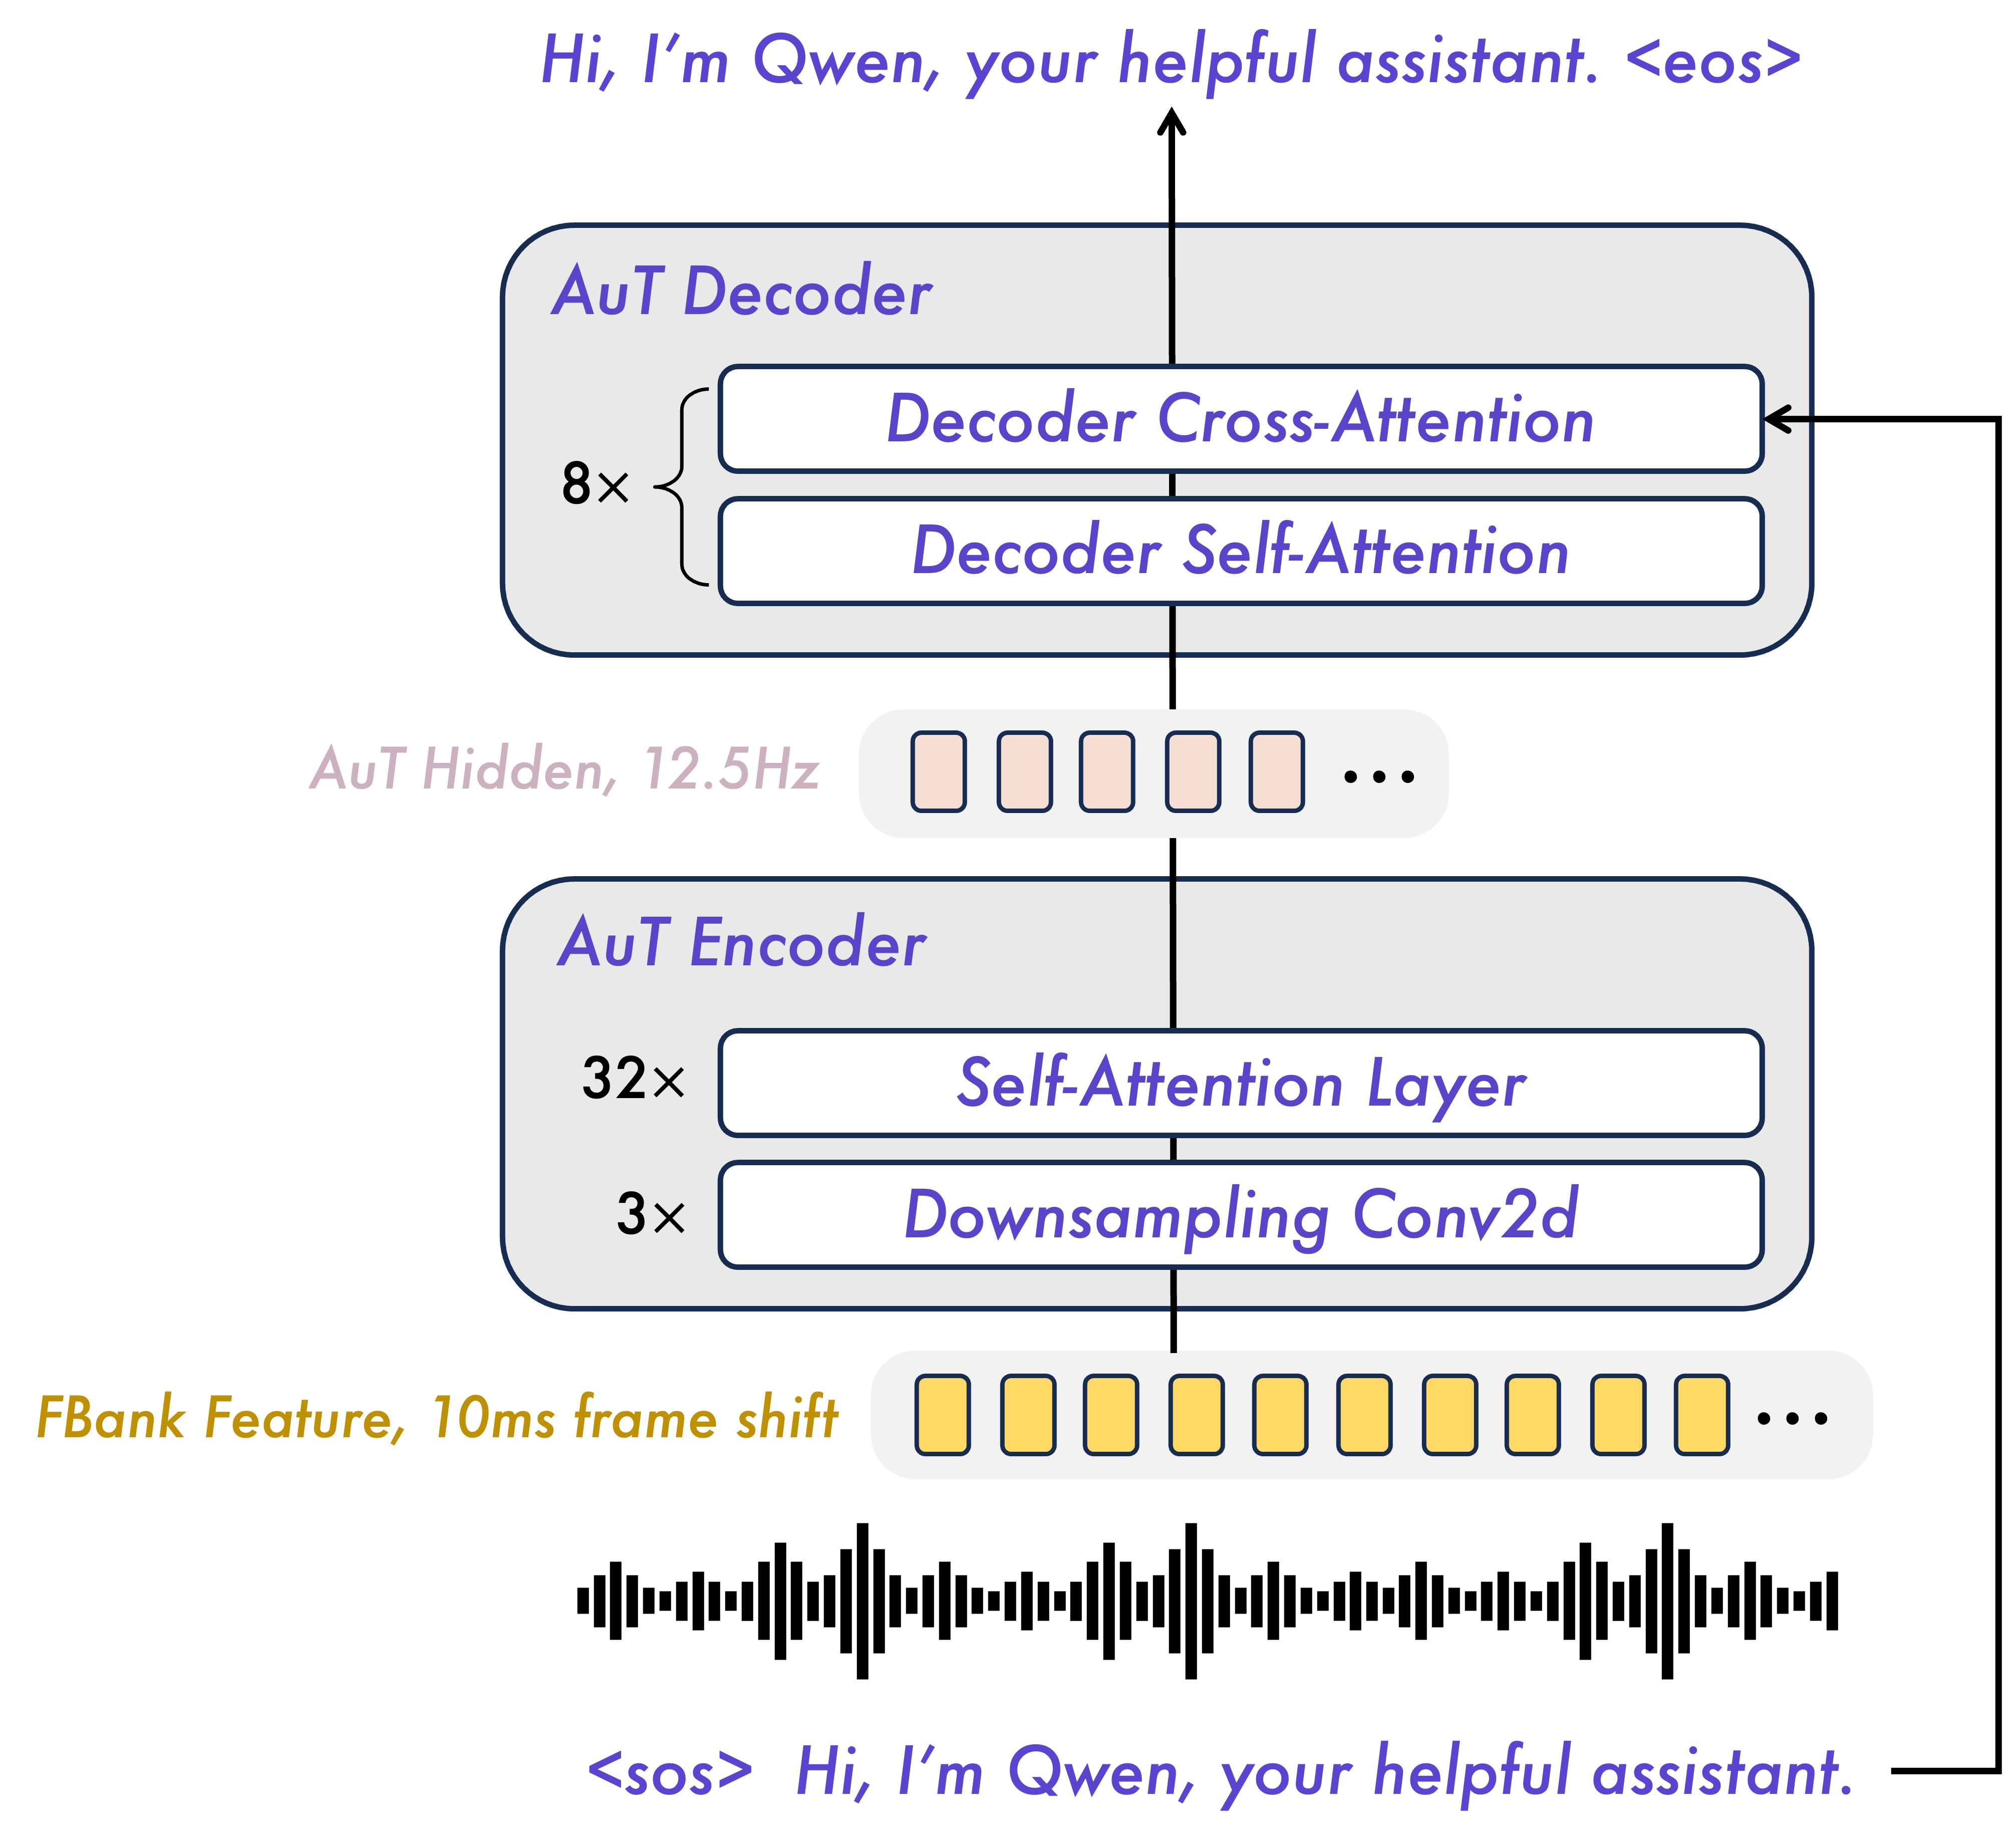
\includegraphics[width=0.6\textwidth]{figures/aut.png}
    \caption{The overview of AuT. AuT is an attention-encoder-decoder based auto-regressive model, which is trained from scratch on 20 million hours of supervised audio. \method employs the AuT encoder as the audio encoder to obtain general purpose audio representations at a token rate of 12.5Hz.}
    \label{fig:aut}
\end{figure}

Audio Transformer (AuT) is an attention-encoder-decoder model, as is shown in Figure~\ref{fig:aut}, trained from scratch on 20 million hours of supervised audio data. During training, the filter bank features of the audio are downsampled 8 times using Conv2D blocks before the attention layers, reducing the token rate to 12.5 Hz. To learn stronger and more general-purpose audio representations, AuT is trained on large-scale audio datasets with both speech recognition and audio understanding tasks. Specifically, the training data includes 80\% Chinese and English pseudo-labeled ASR data, 10\% ASR data from other languages, and 10\% audio understanding data. To balance the efficiency of real-time prefill caching with the performance for offline audio tasks, AuT utilizes flash attention with dynamic attention window sizes, covering attention query patterns ranging from 1 to 8 seconds. In \method, we employ the AuT encoder as the audio encoder, which contains approximately 0.6B parameters.


\subsection{Perceivation}
% \begin{figure}[tbh]
%     \centering
%     
\includegraphics[width=1.0\textwidth]{figures/ATMRoPE.png}
%     \caption{An illustration of Time-aligned Multimodal RoPE~(TMRoPE).}
%     \label{fig:ATMRoPE}
% \end{figure}
\paragraph{Text, Audio, Image and Video (w/o Audio).} 

Thinker converts text, audio, image, and video (without audio) into a series of  representations for input. For text inputs, we use Qwen’s tokenizer~\citep{qwen3}, which applies byte-level byte-pair encoding with a vocabulary of 151,643 regular tokens. For audio inputs and audio extracted from video, we resample to 16 kHz and convert the raw waveform into a 128 channel mel-spectrogram with a 25 ms window and a 10 ms hop. We adopt AuT encoder as our audio encoder, which is trained from scratch on 20 millions hours of audio data, and each frame of the audio representation corresponds to approximately an 80 ms segment of the original audio signal. Furthermore, we employ the vision encoder from Qwen3-VL, initialized from SigLIP2-So400m~\citep{siglip2} with approximately 543 million parameters, enabling handling of both image and video inputs. The vision encoder is trained on a mixture of image and video data, ensuring strong image understanding and video comprehension. To preserve video information as completely as possible while aligning with the audio sampling rate, we sample video frames at a dynamic frame rate.

\paragraph{Video and Multimodal Position Embedding~(TM-RoPE)}  

Drawing inspiration from Qwen2.5-Omni, we employs a Time-aligned Multimodal Rotary Position Embedding (TM-RoPE), which extends the Multimodal Rotary Position Embedding (M-RoPE)~\citep{qwenvl} by incorporating absolute temporal information. TM-RoPE factorizes the conventional rotary position embedding into three distinct dimensions: temporal, height, and width. In the original M-RoPE formulation, temporal dependencies are modeled using the initial 16 rotary angles, which correspond to higher frequencies and exhibit stronger oscillatory patterns. While this design is effective for capturing fine-grained local temporal variations, it can impede the model's ability to extrapolate over extended sequences. To address this limitation, we introduce a modified allocation of rotary angles. Specifically, the temporal, height, and width dimensions are interleaved and assigned 24, 20, and 20 rotary angles, respectively. This redistribution fosters a more balanced representation of both local semantics and long-range dependencies, thereby enhancing the model's overall performance. The application of TM-RoPE is tailored to the specific modality of the input data. For text inputs, the three components share identical position identifiers, rendering TM-RoPE functionally equivalent to a one-dimensional RoPE~\citep{rope}. Similarly, audio inputs utilize shared position IDs but are further augmented with absolute temporal encodings, where each temporal ID corresponds to a duration of 80 ms. For image data, a constant temporal ID is assigned to all visual tokens, while their distinct row and column positions determine the height and width IDs.

In the context of multimodal audiovisual streams, the audio component is encoded with a temporal ID for every 80 ms. The video is treated as a sequence of frames with monotonically increasing temporal IDs that are dynamically adjusted based on their actual timestamps to ensure a consistent temporal resolution of 80 ms per ID. The height and width IDs for video frames are assigned in the same manner as for still images. To prevent positional conflicts when processing multiple modalities, the position numbering is made contiguous, with each subsequent modality commencing from one plus the maximum position ID of the preceding modality. This refined approach to positional encoding enables the model to effectively integrate and jointly model information from diverse modalities. In a departure from Qwen2.5-Omni, which segments audiovisual representations into fixed 2-second chunks, \method directly aligns these representations using their temporal IDs, which are explicitly anchored to absolute time. This design choice affords the model the flexibility to support streaming inputs of arbitrary duration.



\subsection{Speech Generation}
% In multi-turn dialogue, Talker directly inherits the Thinker’s context, including textual tokens and multimodal high-level representations, and synthesizes speech conditioned on the Thinker’s streamed textual output for the current turn. As with text generation, intelligent speech synthesis cannot rely solely on the current query. Long-context representations enable the model to adapt fine-grained acoustic attributes—such as prosody, loudness, and emotion—based on the broader discourse context.

% Unlike~\citet{qwen2.5omni}, Talker operates directly on RVQ tokens produced by \textit{Qwen3-TTS-Tokenizer-v2}. Talker backbone ingests the aggregated codebook features of the current frame and uses a linear head to predict the zeroth codebook. Then, a multi-token prediction (MTP) module then generates the residual codebooks. This design allows Talker to model the full spectrum of fine-grained acoustic detail, thereby enhancing expressivity. Since Talker learns an end-to-end representation over the complete set of codebooks, Code2Wav requires only a causal ConvNet to reconstruct the waveform, achieving substantially lower inference latency and FLOPs while delivering higher fidelity than DiT-based decoders.

For speech synthesis in multi-turn dialogues, our Talker module is conditioned on a rich context inherited from a "Thinker" component, comprising historical textual tokens, multimodal representations, and the current turn's streamed text. This reliance on long-context information is critical, as high-fidelity speech synthesis must adapt acoustic attributes like prosody, loudness, and emotion to the ongoing discourse, a principle well-established in context-aware generative models.

Architecturally, our approach departs from~\citet{qwen2.5omni} by operating directly on RVQ tokens. The Talker employs a hierarchical prediction scheme: the backbone ingests the aggregated codebook features of the current frame and uses a linear head to predict the zeroth codebook, after which a multi-token prediction (MTP) module generates all residual codebooks. This strategy enables the model to learn a complete representation of acoustic details, enhancing vocal expressivity. Consequently, waveform reconstruction is simplified to a lightweight causal ConvNet (Code2Wav), which significantly reduces inference latency and computational cost (FLOPs) while achieving superior audio fidelity compared to more complex DiT-based vocoders.

\subsection{Designs for Streaming and Concurrency}
In streaming audiovisual interaction scenarios, the first-packet latency is a critical factor affecting user experience, and the model's concurrency capability is key to reducing service costs and improving response speed. This section discusses how \method enhances concurrency and reduces first-packet latency through algorithmic and architectural optimizations.

\begin{table}[htbp]
\centering
\caption{\textbf{The architectural design of Qwen3-Omni-30B-A3B and the end-to-end first-packet latency for Audio/Video~(ms).}}
\vspace{-1mm}
\begin{tabular}{lccc}
\toprule
\textbf{Module}         & \textbf{Architecture}      & \textbf{Params}    & \textbf{Streaming} \\\midrule
Audio Encoder  & AuT               & 650M      & $\checkmark$        \\
Vision Encoder & SigLIP2-So400M    & 540M     & -        \\
Thinker        & MoE Transformer   & 30B-A3B  & $\checkmark$        \\
Talker         & MoE Transformer   & 3B-A0.3B & $\checkmark$        \\
MTP            & Dense Transformer & 80M     & $\checkmark$        \\
Code2wav       & ConvNet           & 200M     & $\checkmark$        \\\midrule
\multicolumn{4}{c}{End-to-End First-Packet Latency: \textbf{234/547ms}} \\
\bottomrule
\end{tabular}
\end{table}


\paragraph{Chunked Prefilling and MoE Architecture.} In \method, we retain the chunked-prefilling mechanism as implemented in Qwen2.5-Omni, whose audio and vision encoders are capable of outputting chunks along the temporal dimension. During real-time interaction, Thinker and Talker modules perform asynchronous prefilling: when Thinker completes prefilling the current chunk, its output high-level representations are immediately used to prefill the Talker’s current chunk asynchronously, while Thinker prefills its next chunk. This approach significantly reduces the Time-To-First-Token (TTFT) for both the Thinker and the Talker. Architecturally, both Thinker and the Talker in \method adopt the MoE design, which is highly effective for improving service throughput. Compared to dense models, the MoE architecture significantly decreases IO consumption arising from KV cache during processing of long sequences, thereby increasing tokens per second (TPS) during generation and enhancing concurrency.

\paragraph{Streaming Multi-Codebook Codec Generation.} To minimize the user's waiting time for receiving the first generated packet, we propose a \textit{left context only multi-codebook generation} mechanism. As shown in Figure~\ref{fig:ovewview_arch}, once Talker generates the first token, the MTP module predicts the remaining tokens for the current frame. These tokens are then decoded into waveform by a streaming multi-codebook codec decoder that only attends to the left context. Unlike Qwen2.5-Omni that requires waiting for sufficient block-context from the Talker before synthesis, \method can output the waveform immediately after the Talker generates each token, significantly reducing first-packet latency. 

\paragraph{Lightweight MTP module and ConvNet.} Both the MTP module and codec decoder are lightweight modules, which have low computational FLOPs and support batched inference, making them well-suited for high-concurrency scenarios. The MTP Module is an ultra-lightweight fixed-step autoregressive dense transformer, with low memory bandwidth requirements on inference hardware, thereby naturally enabling efficient batch processing of high throughput requests. Its fixed-step autoregressive inference mechanism allows it to effectively leverage a fixed KV cache memory space for acceleration, achieving low inference latency. Meanwhile, the ConvNet-based codec decoder also achieves high throughput with low latency because its convolutional architecture enjoys extensive hardware acceleration support across diverse inference platforms, and it enables efficient batched inference.

\begin{table}[htbp]
\centering
\caption{\textbf{Theoretical First-Packet Latency of \method wit Different Concurrency.}}
\label{tab:inference-lantency}
\small
\setlength{\tabcolsep}{2.6pt}
\begin{tabular}{@{}lccc@{}}
\toprule
 & \multicolumn{3}{c}{\textbf{\method-30B-A3B}} \\
\cmidrule(lr){2-4}
 & \textbf{1 Concurrency} & \textbf{4 Concurrency} & \textbf{6 Concurrency} \\
\midrule
Thinker-Talker Tail Packet Preprocessing Latency & 72/160ms & 94/180ms & 100/200ms \\
Thinker Time-to-First-Token (TTPT) & 88/160ms & 468/866ms & 673/1330ms \\
Talker Time-to-First-Token (TTPT) & 57/210ms & 145/450ms & 376/734ms \\
MTP Module Time Cost Per Token & 14ms & 16ms & 18ms\\
Codec Decoder Time Cost Per Code & 3ms & 5ms & 5ms \\
\midrule
\textbf{Overral Latency~(Audio/Video)} & \textbf{234/547ms} & \textbf{728/1517ms} & \textbf{1172/2284ms} \\
\midrule
Thinker Token Generation Rate (TPS) & 75 tokens/s & 63 tokens/s & 53 tokens/s \\
Talker Token Generation Rate (TPS) & 140 tokens/s & 125 tokens/s & 110 tokens/s \\
\midrule
\textbf{Generation RTF(Real Time Factor)} & \textbf{0.47} & \textbf{0.56} & \textbf{0.66} \\
\bottomrule
\end{tabular}
\end{table}


Table~\ref{tab:inference-lantency} presents the theoretical first-packet latency for \method under typical computational resources across varying concurrency scenarios. Experiments are conducted on the vLLM framework~\citep{vllm} to process concurrent audiovisual streams, with optimizations applied via \textit{torch.compile} and CUDA Graph acceleration to the MTP Module and codec decoder. Several factors influence the total first-packet latency. First, the model sizes of Thinker and Talker impact their tail packet preprocessing latency (multi-modal data preprocessing and inference for Audio and Vision Encoder) and Time-To-First-Token (TTPT). Second, the architectures and sizes of the MTP Module and Codec Decoder affect their inference latency. Due to the sequential dependency between these components, the total first-packet latency represents the sum of these individual latencies. As shown in the results, the MoE architecture of Thinker and Talker ensures that their prefill latency and TTPT remain largely unaffected under high concurrency. Meanwhile, the lightweight design of the MTP Module and Codec Decoder minimizes their computational overhead, resulting in a lower impact on first-packet latency. Furthermore, after the initial packet is output and the model starts streaming audio synthesis, the 12.5Hz token rate Talker requires only one token to synthesize 80ms audio. Consequently, the Generation Real Time Factor (RTF) is calculated by dividing the sum of:  (1) the time taken by Thinker and Talker to generate one token; and (2) the processing time per token for the MTP Module and Codec Decoder by 80ms. As demonstrated, the RTF consistently remains below 1 across varying concurrency levels, ensuring that users receive continuously streaming audio responses.



% \paragraph{Large Thinker and Small Talker.} To reduce the computational cost and latency, we use a small Talker, xxx M.


% For tokenization, we utilize Qwen's tokenizer~\citep{qwen}, which implements byte-level byte-pair encoding (BBPE,~\citealp{gpt3,wang2020neural,sennirch2016neural}) with a vocabulary of 151,643 regular tokens. We have expanded the set of control tokens from 3 to 22 compared to previous Qwen versions, adding two new tokens for tool functionality and allocating the remainder for other model capabilities. This expansion establishes a unified vocabulary across all Qwen2.5 models, enhancing consistency and reducing potential compatibility issues.

% \begin{table}[tbp]
% \caption{Model architecture and license of Qwen2.5 open-weight models.}
% \small
% \centering
% \begin{tabular}{@{}lcccccccc@{}} 
% \toprule
% Models  & Layers & Heads (Q / KV) & Tie Embedding & Context / Generation Length  & License \\
% \midrule
% 0.5B  & 24 & 14 / 2 & Yes & 32K / 8K & Apache 2.0 \\
% 1.5B  & 28 & 12 / 2 & Yes & 32K / 8K & Apache 2.0 \\
% 3B  & 36 & 16 / 2 & Yes & 32K / 8K & Qwen Research \\
% 7B  & 28 & 28 / 4 & No & 128K / 8K & Apache 2.0 \\
% 14B & 48 & 40 / 8 & No & 128K / 8K & Apache 2.0 \\
% 32B & 64 & 40 / 8 & No & 128K / 8K & Apache 2.0 \\
% 72B  & 80 & 64 / 8 & No & 128K / 8K & Qwen \\
% \bottomrule
% \end{tabular}
% \end{table}
